\chapter{Introduction to the course}
\section{Overview of the course}

\begin{itemize}
\item \side{\textbf{Real time systems}}

About the topic we will cover:
\begin{itemize}
\item \side{Real-Time Computing} and \side{temporal constraints}\\
Real time systems are software and hardware systems (hence computing systems), that have to comply with temporal constraints.
\item Definitions and task model\\
We will make things much clearer and better defined by introducing a sequence of definitions and mathematical models that will allow us to given this notion of temporal constraint a well founded meaning .
\item \side{Real Time Scheduling}\\
We will also study solutions that allow us to enforce these real time constraints and this solution will have much to do on how we schedule shared resources.
\end{itemize}

\item \side{\textbf{POSIX API}}\\
We will move to a concrete ground and see what is the exact shape that these notions take once they are moved in a computer program. 
\item \side{\textbf{Real-Time Scheduling}}\\
As regards the Real-Time scheduling we will see many interesting policies, but since this is  not a course on Real Time scheduling what we will do is provide the knowledge of real time scheduling so that the reader will be able to understand the mechanism of real time operating systems and thereby make best use of these technologies in future projects.
\item \side{\textbf{Operating System structure}}\\
Since it will be important to keep in check the latencies, we will cover:
\begin{itemize}
\item Notes about traditional kernel structures.\\
In order to keep latencies in check, we need proper technological solutions that make our operating systems differ quite a bit from standard operating systems.
\item Sources of kernel latencies.\\
\item Some approaches to real-time kernels (e.g dual kernel approach, interrupt pipes, microkernels, monolithic kernels and RT). 
\end{itemize}
\item \side{\textbf{Real-Time Kernels and OSs}}
\item \side{\textbf{Developing Real-Time applications}}
\end{itemize}

\section{Real-Time Systems}
In order to discuss about the Real-Time systems we need to provide some basic definitions:
\begin{itemize}
\item{\makebox[6cm]{Real-Time Operating Systems (RTOS)\hfill} is an operating system providing support to Real Time applications}\pside{Real-Time Operating Systems (RTOS)}
\item{\makebox[6cm]{Real-Time Application\hfill} the correctness of the application does not only depends on the output values/results that the application produces, but also on the time when such values are delivered}\pside{Real-Time Application}
\item{\makebox[6cm]{Operating System\hfill} an operating systems can be looked at from many different perspective:}\pside{Operating System (OS)}
\begin{enumerate}
\item Set of computer programs, of critical programs to be precise: because they have to be written efficiently, otherwise the hardware resources get disrupted, hence the system cannot operate correctly.
\item Interface between applications and hardware. 

Whenever an application interacts with an hardware, it is not of the developer interest to directly control the hardware. The Operating System provides an API that enables you to open a connection to a peripheral and takes care of all the low level interactions.
On this regard, understanding the notion of \side{interrupt} will be of fundamental importance, because it is, essentially, what gave rise to concurrent programming: in the case we would like to interact with a peripheral, rather than continuously check if the peripheral has ended what it is supposed to do, you can tell the peripheral to communicate when it has completed the given task.

Anyway the Operating systems acts as an interface towards the hardware and hides away all these complex details.
\item Control the execution of application programs.
\item Manage the hardware and software resources.
\end{enumerate}
\end{itemize}

\subsection{Real-Time Operating Systems}

Since the OS is something that lies in-between the user application and the hardware resources we can summarize the aforementioned interpretation of the OS, as:
\begin{itemize}
\item \side{Service Provider} for user programs (i.e. exports a programming interface).

This concept looks at the OS from the perspective of the software application.
\item \side{Resource Manager} (i.e. implements schedulers)

This concept looks at the OS from the perspective of the hardware.
\end{itemize}

\subsubsection{OS as a Service Provider}
One way of looking at the OS is as a Service Provider, in the sense that it provides:
\begin{itemize}
\item Process Synchronization mechanism
\item Inter-Process Communication (IPC)
\item Process/Thread Scheduling, i.e.  ways to create and schedule tasks
\item Input/Output
\item Virtual Memory
\end{itemize}
And all these services are accessible through an API.
\subsubsection{OS as a Resource Manager}

If you think at the Operating System as a Resource Manager, then it is something that takes care of many things:
\begin{enumerate}
\item \side{Process Management}\\
The fact that multiple applications can run at the same time on a PC, even though there is a small amount of processor available to manage these applications. (generally 2,4 or 8).

The number of application that you are likely to create is often on the hundreds, hence it is necessary to make an appropriate sharing of the limited resources that you have in order for all the applications to live correctly.
\item \side{Memory Management}\\
Supposing one is using a 64-bit architecture, what will happen is that a space of memory is addressable with 64 bit. As a consequence we can imagine that the addressable memory is space has $2^{64} - 1$ memory locations available.

And each application sees, these much space available for its execution. But however large the space can be in a machine, it will never match the aforementioned size. It could potentially for one task, but in the case a machine is hundreds of tasks and each of them wants to use that much memory, there is no way that the hardware can provide enough physical memory to satisfy all of them.

To counteract this problem, it is common practice to schedule the memory as well, because you take advantage of the fact that an application CAN use $2^{64} - 1$ memory locations, but at a given time it uses a tiny portion of these locations. It is only that tiny portion of memory locations that needs to be made available to the running task.

In this scenario, the OS makes it possible to accommodate within the physical memory of the computer these small slices of the available space that the application uses. So somehow it operates as a resource manager for the memory as well.
\item \side{File Management}
\item \side{Networking}, \side{Device Drivers}, \side{Graphical Interface}
\end{enumerate}
The important thing is that all of these resources, like the processor, the memory, the drivers etc..., are shared between all the tasks.
All these resource managers have to be distributed among all the spectrum of tasks in such a way that the tasks behave properly, i.e. if you do not provide frequently enough these resources they would not be able to deliver the result on time (the OS manages this problem on its own).

In the case we decide to look at the Operating System as a Resource Manager, we need to think of a structure for the OS that makes this resource management effective, effective in the sense that we believe it is the most relevant for our specific range of application.

The way OSs handles devices, interrupt, etc. can be very different (and optimized in very different ways) depending on the type of application one is looking at. However, the type of optimizations we are interested in are those that allow our application to have time-limited execution.

\subsection{Real-Time Concepts and Definitions}
A \side{Real-Time application} is an application of which the time when a result is produced matters.

In particular:
\begin{itemize}
\item a correct result produced too late is equivalent to a wrong result, or to no result.
\item it is characterized by temporal constraints that have to be respected.
\end{itemize}

Example: let us consider a mobile vehicle with a software module that 
\begin{enumerate}
\item Detects obstacles 
\item Computes a new trajectory to avoid them
\item Computes the commands for engine, breaks, ...
\item Sens the commands
\end{enumerate}
If you decide to steer to the left or to the right there is a limited amount of time in which the operation has to be carried out. Hence if one can find an extremely effective strategy for steering the wheels but the strategy amounts to setting the values for the motors after one second, it is completely useless, since the vehicle is most likely to crash.

Hence a time violation in executing a task is a critical problem: it means that the developed application is useless and also dangerous.

But then, what is a reasonable time frame for completing the steering operation?\\
Depends on the speed in which the vehicle is traveling. But no matters if the vehicle is traveling at high or low speed the timing constraint is there, and if it is violated, the vehicle will eventually crash against the obstacle.

As a consequence: when a constraint is set, that constraint needs to be respected. And this is one of the core concept of Real Time:
it is not necessarily synonym of fast execution, but rather of \side{predictable} execution.

Real time computing has much more to do with predictability than of being quick.

Examples of temporal constraints could be:
\begin{itemize}
\item must react to external events in a predictable time
\item must repeat a given activity at a precise rate
\item must end an activity before a specified time
\end{itemize}
In this case, we can clearly notice that the temporal constraints can be either one shot events or periodic events, but in both cases, a common characteristic, there is a need of being predictability.

Temporal constraints are modeled using the concept of \side{deadline}.

\subsubsection{Real-Time \& Determinism}
A Real-Time system is not just a ``fast system'', because the speed is always relative to a specific environment, i.e. the steering commands temporal constraint is set by the velocity of the vehicle.

Running faster is good, but does not guarantee the correct behavior. In fact, it is far more valuable to that temporal constraints are always respected; in other terms Real time systems prefer to run fast enough to respect the deadlines, to be reliable.

Hence, the type of analysis that is necessary to perform is not an analysis based on of average/typical cases but rather an analysis of worst case: I have to prove that even in the worst-case scenario, there is not deadline violation.

\subsubsection{Throughput vs Real-Time}
This predictability creates a wide gap between what a Real Time system is and what a general purpose system is, because general purpose systems are optimised for the average case, but a real time system only cares about the worst case. As a consequence, the way one designs a Real Time system is very different from the way a general purpose system is designed.

In fact:
\begin{itemize}
\item When one optimize for the average case, what one would look at is the number of times that an application completes a task every second, and this is called \side{Throughput}.
\item When one have a worst case requirement, the notion of throughput is not relevant anymore, and the analysis focuses in every single instance the maximum delay will be bounded.
\end{itemize}

\subsubsection{Processes, Threads and Tasks}
Let us introduce some notion and general terms that we will extensively using during the course
\begin{itemize}
\item{\makebox[2cm]{Algorithm\hfill}logical procedure used to solve a problem}\pside{Algorithm}
\item{\makebox[2cm]{Program\hfill}formal description of an algorithm, using a programming language}\pside{Program}
\item{\makebox[2cm]{Process\hfill}Instance of a program (program in execution)}\pside{Process}
\item{\makebox[2cm]{Thread\hfill}flow of execution, something that is able to execute using your processor along with other threads. These threads can be part of the same program and they can be executed in parallel.}\pside{Thread}
\item{\makebox[2cm]{Task\hfill}process or thread}\pside{Task}
\end{itemize}

Hence there are two different ways of sharing resources: one are threads in which your share computing resources and memory space, and processes in which you share computer resources but each of the processes has its own memory space.

Unfortunately, there is no common definition of a task: somebody use the terms with the same meaning as a thread and sometimes it is used with the same meaning as a process. In this class we will refer to threads.

Henceforth, when we talk about a task we will refer to a program that it is running and they share the same memory space with other programs.

\section{Real-Time Tasks}
A task can be seen as a sequence of actions and a deadline must be associated to each one of them.

We, therefore, are after is a definition of a formal model that identifies what these tasks or actions are and associate deadlines with them. 
\subsection{Mathematical Model of a Task}
We can define a \side{Real-Time task} $\tau_i$ as a stream of jobs or instances $J_{i,k}$. In other terms, it is a sequence of activity that is activated periodically or aperiodically.

Each job $J_{i,k} = (r_{i,k}, c_{i,k}, d_{i,k})$, that is characterized by a tuple of four values:
\begin{itemize}
\item{\makebox[2cm]{$r_{i,k}$\hfill}instant when the job is activated}
\item{\makebox[2cm]{$c_{i,k}$\hfill}computation time}\pside{computation time}
\item{\makebox[2cm]{$d_{i,k}$\hfill}absolute deadline}\pside{absolute deadline}
\item{\makebox[2cm]{$f_{i,k}$\hfill}finishing time (of the computation), which has to be smaller than the absolute deadline}\pside{finishing time}
\end{itemize}

Furthermore, since each task $i$ is a sequence of jobs, we need to differentiate between them. That is why each job $J_{i,k}$ is uniquely identified by its task index $i$ and the $k$-th activation of the $i$-th task.

\begin{figure}[!h]
\centering
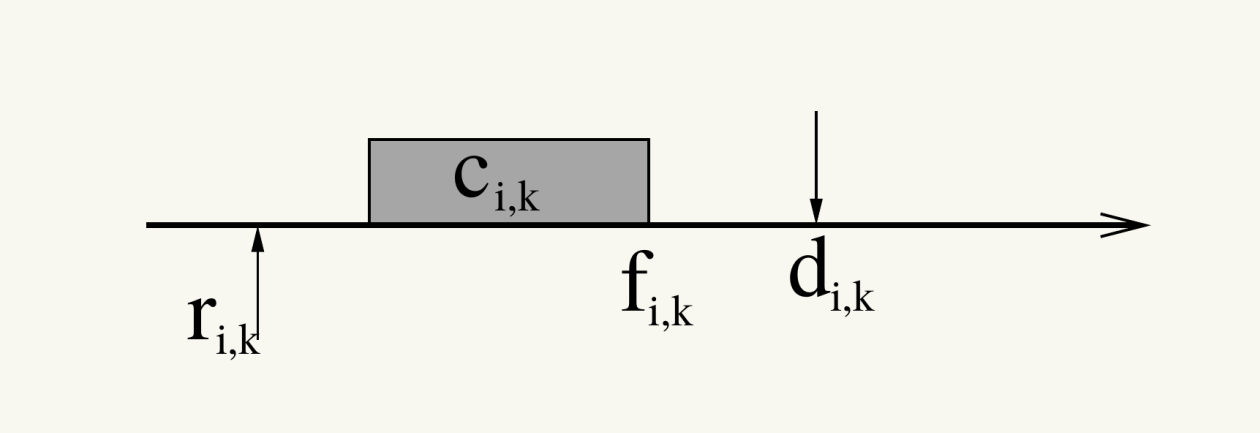
\includegraphics[width= .65\textwidth]{image01}
\end{figure}

Formally:
A job is an abstraction used to associate deadlines (temporal constraints) to activities
\begin{itemize}
\item $r_{i,k}$ time when job $J_{i,k}$ is activated (by an external event, a timer, an explicit activation, etc..)
\item $c_{i,k}$ computation time needed by job $J_{i,k}$ to complete
\item $d_{i,k}$ absolute time instant by which job $J_{i,k}$ must complete 

job $J_{i,k}$ respects its deadline if $f_{i,k} \le d_{i,k}$
\item \side{Response time} of job $J_{i,k}$
\[\rho_{i,k} = f_{i,k} - r_{i,k}\]
\end{itemize}

\subsection{Periodic Tasks}
A \side{Periodic Task} is uniquely represented by a tuple of three values in the form:
\[\tau_i = (C_i, D_i, T_i)\]
and it represents a stream of jobs $J_{i,k}$ with:
\begin{align*}
r_{i,k+1} &= r_{i,k} + T_i\\
d_{i,k} &= r_{i,k}  + D_i\\
C_i &= \max_{k}\{c_{i,k}\}
\end{align*}
where
\begin{itemize}
\item{\makebox[0.5cm]{$T_i$\hfill} is the task }\side{period}
\item{\makebox[0.5cm]{$D_i$\hfill} is the task }\side{relative deadline}
\item{\makebox[0.5cm]{$C_i$\hfill} is the task }\side{worst-case execution time (WCET)}
\item{\makebox[0.5cm]{$R_i$\hfill} is the task }\side{worst-case response time (WCRT)} defined as
\[R_i = \max_k\{\rho_{i,k}\} = \max_k\{f_{i,k} - r_{i,k}\}\]
\end{itemize}
For the task to be correctly scheduled, it must hold that:
\[R_i \le D_i\]

A periodic task has a regular structure (called \side{cycle}), in the sense that:
\begin{enumerate}
\item it is activated periodically with a period of $T_i$
\item it executes a computation
\item when the computation terminates, it suspends waiting for the next period
\end{enumerate}

Hence, its fundamental implementation can be represented as:

\begin{lstlisting}[language=C++]
void *PeriodicTask(void *arg)
{
	<initialization>;
	<start periodic timer, period = T>;
	while (condition)
	{
		<read sensors>;
		<update outputs>;
		<update state variables>;
		<wait next activation>;
	}
}
\end{lstlisting}

Tasks are graphically represented by using a \side{scheduling diagram}. For instance, figure \ref{fig:perta} shows a schedule of a periodic task 

\begin{gather*}
\tau_1 = (3,6,8)\\
WCET_1 = 3\quad D_1 = 6\quad T_1 = 8
\end{gather*}

\begin{figure}[!h]
\centering
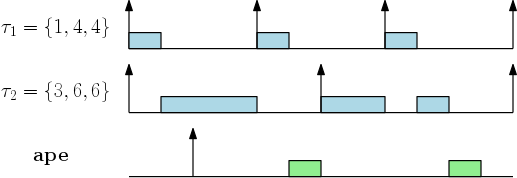
\includegraphics[width=.8\textwidth]{image02}
\caption{Periodic task graphical representation}
\label{fig:perta}
\end{figure}

Notice that, while job $J_{1,1}$ and $J_{1,3}$ execute for 3 units of time (WCET), job $J_{1,2}$ executes for only 2 units of time.

\subsection{Aperiodic Tasks}
\side{Aperiodic Task}s are not characterised by periodic arrivals, meaning that
\begin{itemize}
\item A minimum interarrival time between activations does not exist
\item Sometimes, aperiodic tasks do not have a particular structure
\end{itemize}
However, aperiodic tasks are of fundamental importance given that they model:
\begin{enumerate}
\item Tasks responding to events that occur rarely (e.g. a mode change)
\item Tasks responding to events with irregular structure (e.g. bursts of packets from the network, ...)
\end{enumerate}

A possible pattern for an aperiodic task $\tau_1$ is proposed in figure \ref{fig:aperta}

\begin{figure}[!h]
\centering
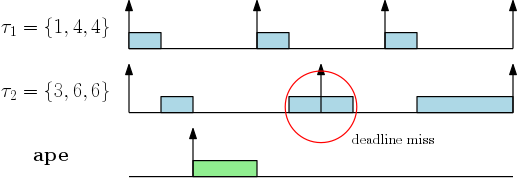
\includegraphics[width=.8\textwidth]{image03}
\caption{Aperiodic task graphical representation}
\label{fig:aperta}
\end{figure}
notive that arrivals might be bursty, and there is not a minimum time between them

\subsection{Sporadic Tasks}
\side{Sporadic Task}s are aperiodic tasks characterised by a minimum interarrival time between jobs. In this sense, they are similar to periodic tasks, but while a periodic task is activated by a periodic timer, a sporadic task is activated by an \side{external event} (e.g. the arrival of a packet from the network)

Hence, its fundamental implementation can be represented as:
\begin{lstlisting}[language=C++]
void *SporadicTask(void *arg)
{
	<initialization>;
	while (condition)
	{
		<computation>;
		<wait events>;
	}
}
\end{lstlisting}

Given its similarity with periodic task, a sporadic task can be represented by a tuple of three values
\[\tau_i = (C_i, D_i, T_i)\]
and it represents a stream of jobs $J_{i,k}$ with 
\begin{align*}
r_{i,k+1} &\ge r_{i,k} + T_i\\
d_{i,k} &= r_{i,k} + D_i\\
C_{i} &= \max_k \{c_{i,k}\}
\end{align*}
where
\begin{itemize}
\item{\makebox[0.5cm]{$T_i$\hfill} is the task }\side{minimumm interarrival time (MIT)}
\item{\makebox[0.5cm]{$D_i$\hfill} is the task relative deadline}
\item{\makebox[0.5cm]{$C_i$\hfill} is the task worst-case execution time (WCET)}
\end{itemize}
The task is correctly scheduled if $R_i \le D_i$

Since sporadic task can be represented by a mathematical model, they can be graphically displayed. Hence, figure \ref{fig:sporata} shows a possible schedule of a sporadic task $\tau_1 = (2,5,9)$.

\begin{figure}[!h]
\centering
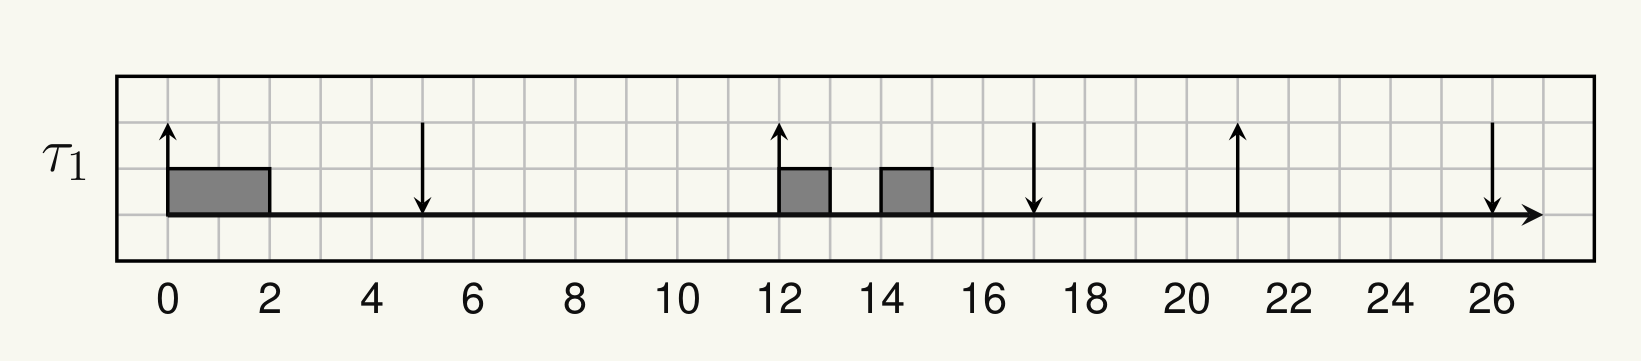
\includegraphics[width=.8\textwidth]{image04}
\caption{Sporadic task graphical representation}
\label{fig:sporata}
\end{figure}

Notice that
\begin{align*}
r_{1,2} &= 12 > r_{1,1} + T_1 = 9\\
r_{1,3} &= 21 = r_{1,2} + T_1 = 21
\end{align*}

\section{Task Criticality}
A deadline is said to be \side{hard} if  deadline miss causes a critical failure in the system, whereas a task is said to be a \side{hard real-time task} if all its deadlines are hard, which means that all the deadlines must be guaranteed before starting the task, i.e.
\[\forall j, \rho_{i,j} \le D_i \qquad\Rightarrow\qquad R_i \le D_i\]

Example:

The controller of a mobile robot, must detect obstacles and react within a time dependent on the robot speed, otherwise the robot will crash into the obstacles

A deadline is said to be \side{soft} if a deadlien miss causes a degradation in the \side{Quality of Service (QoS)}, but is not a catastrophuc event, whereas a task is said to be a \side{soft real-time task} if it has soft deadlines.

In other terms, some deadlines can be missed without compromising the correctess of the system, but the number of missed deadlines must be kept under control, because the \emph{quality} of the results depend on the number of missed deadlines.

Unline the hard real-time task, soft real-time tasks can be difficult to characterize, particularly:
\begin{itemize}
\item What's the tradeoff between ''non compromising the system correctness'' and not considering missed deadlines?
\item Moreover, some way to express the QoS experienced by a soft real-time task is needed
\end{itemize}

Exmplaes of QoS definitions could be
\begin{itemize}
\item no more than X consecutive deadlines can be missed
\item no more that X deadlines in an interval of time $T$ can be missed
\item the \side{deadline miss probability} must be less than a specified value, i.e.
\[P\{f_{i,j} > d_{i,j}\} \le R_{max}\]
\item the \side{deadline miss ratio} must be less than a specified value, i.e.
\[\cfrac{\text{number of missed deadlines}}{\text{total number of deadlines}} \le R_{max}\]
\item the maximum \side{tardiness} must be less than a specified value, i.e.
\[\cfrac{R_i}{D_i} < L\]
\item ...
\end{itemize}

A common example of implementation of a soft real-time task are the Audio and Video players. Particularly, assuming a framerate of 25 fps, which imply a frame period of 40 ms, if a frame is played a little bit too late, the user might even be unable to notice any degration in the QoS, however, \side{skipped frames} can be disturbing.

In fact missing a lot of frames by 5 ms can be better than missing only a few frames by 40 ms.

Another common example, can be found in some robotic systems where some actuations can be delayed with little consequences on the control quality.

In any case, soft real-time constraints does not mean no guarantee on dealines, given that tasks can have variable execution times between different jobs.\\
These execution times might depend on different factors:
\begin{itemize}
\item Input data
\item HW issues (cache effects, pipeline stalls, ...)
\item The internal state of the task
\item ...
\end{itemize}





















